\documentclass{beamer}

\usepackage{hyperref}
\usepackage{tabulary}
\usepackage{multirow}
\usepackage{booktabs}

\usetheme{metropolis}

\title{Guide for \texttt{thesisdtetiugm} Class File}
\subtitle{Introduction to \texttt{thesisdtetiugm}}

\author{Muhammad Yasirroni}
\institute{Universitas Gadjah Mada}
\date{\today}

\begin{document}

\begin{frame}
  \titlepage
\end{frame}

\section{Introduction}
\begin{frame}
    \frametitle{Why thesisdteti?}
    \begin{itemize}
      \item LaTeX is based on the idea that it is better to leave document design to document designers, that is the community maintaining thesisdteti class file.
      \item Authors should focus only with the writing of the documents.
      \item Open source class file allows everyone, including authors, to contribute back and improve the class file.
    \end{itemize}
\end{frame}

\begin{frame}
  \frametitle{Where is \texttt{thesisdtetiugm}?}
  \texttt{thesisdtetiugm} is available at GitHub repository (\href{https://github.com/yasirroni/thesisdtetiugm}{here}). Altough it is more recommended to use Git to stay updated, a static \texttt{.zip} file is available (\href{https://github.com/yasirroni/thesisdtetiugm/archive/refs/heads/master.zip}{here}).
\end{frame}

\section{Document Class}

\begin{frame}[fragile]
  \frametitle{Document Class Options}

  \textbf{Default Setting}

  \begin{block}{}
    \vspace{-2em}
    \small
    \begin{verbatim}
\documentclass[master,bahasa,table,xcdraw]{thesisdtetiugm}
    \end{verbatim}
  \end{block}

  \textbf{Setting Options}

  \begin{itemize}
    \item \texttt{<bachelor/master/doctoral>}: degree
    \item \texttt{<bahasa/english>}: language
    \item \texttt{<table>,<xcdraw>} (optional): supports coloring table
  \end{itemize}

\end{frame}

\section{External Files}

\begin{frame}[fragile]
  \frametitle{\texttt{input} and \texttt{output}}

  \verb|\input|

  The \verb|\input{PATH/TO/FILENAME.tex}| inserts valid LaTeX code from the specified file.

  \vspace{\baselineskip}

  \verb|\include|

  The \verb|\include{PATH/TO/FILENAME.tex}| inserts valid LaTeX code from the specified file by inserting on different page. \verb|\include| allows the use of \verb|\includeonly| to specify list of file that will be included upon rendering.
\end{frame}

\begin{frame}[fragile]
  \frametitle{Figures}

  \textbf{Using} \verb|\includegraphics|

  \begin{block}{}
    \vspace{-2em}
    \small
    \begin{verbatim}
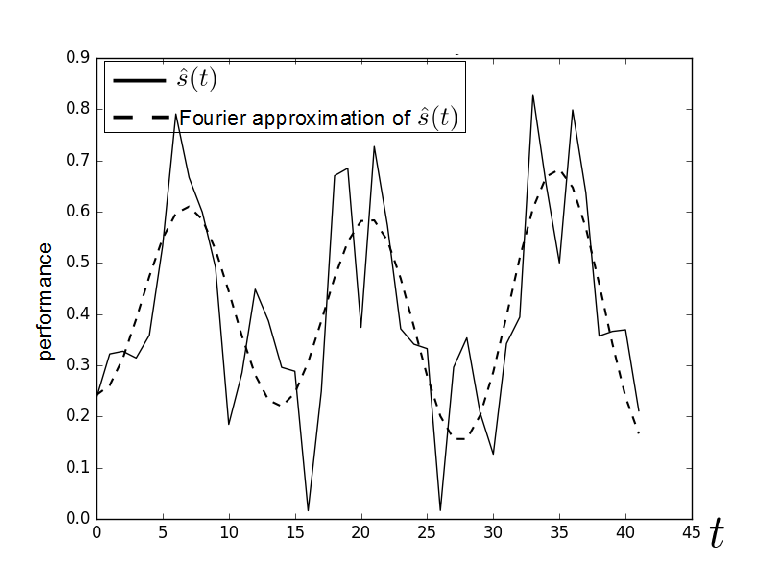
\includegraphics[width=10cm]{images/sample-fig.png}
    \end{verbatim}
  \end{block}

  \textbf{Setting} \verb|\includegraphics|

  \begin{itemize}
    \item \verb|<width=WIDTHcm>| (optional): adjust the width of the image 
    \item \verb|<FILE_NAME>.ext|: the extension supports various type such as \texttt{.png}, \texttt{.jpg}, and even \texttt{.pdf}. 
  \end{itemize}

  It is more recommended to not using both \texttt{<height>} and \texttt{<scale>} parameters. Stick with known \texttt{<width>} or page area for the images and let the document decides the height. Alternatively, not using any parameter is also possible to let LaTeX decides the resize.

\end{frame}

\begin{frame}[fragile]
  \frametitle{Codes}

  \textbf{Using} \verb|\lstinputlisting|

  \begin{block}{}
    \vspace{-2em}
    \small
    \begin{verbatim}
\lstinputlisting[%
  language=Python,%
  caption={CAPTION \textit{SUPPORT ITALIC}.},%
  label={lst:FILE_NAME}]%
  {codes/FILE_NAME.py}
    \end{verbatim}
  \end{block}

\end{frame}

\begin{frame}[fragile]
  \frametitle{Equations}

  \textbf{Using a Custom Function of} \verb|\inputeq|

  \verb|\inputeq| is a custom command to import equation from separate file. The downside of this function is it uses multiple calls of open, read, and find to look for the equation, making the compilation slightly slower but almost negligible. Read \texttt{main/equations/equations.tex} for the detail of the syntax in creating your own \texttt{equations.tex} file.

  \textbf{Syntax for} \verb|\inputeq|

  \begin{block}{}
    \vspace{-2em}
    \small
    \begin{verbatim}
\inputeq{equations/equations}{miqp-obj}
    \end{verbatim}
  \end{block}

\end{frame}

\section{Tables}
\begin{frame}
  \frametitle{Default Table}

  \begin{table}[h]
    \centering
    \caption{Tabel Tinggi Berat}
    \begin{tabular}{|c|c|c|c|c}
      \hline
      ID & \multicolumn{2}{c}{Laki-laki} & \multicolumn{2}{c}{Perempuan} \\
      \hline
       & Tinggi Badan (cm) & Berat Badan (kg) & Tinggi Badan (cm) & Berat Badan (kg) \\
      \hline
      A23   & 173 & 62  & 173 & 62 \\ \hline
      A25   & 185 & 70  & 185 & 70 \\ \hline
      A10   & 162 & 78  & 162 & 78 \\ \hline
      Total & 520 & 210 & 520 & 210 \\ \hline
    \end{tabular}
    \label{tab:tinggiberat}
  \end{table}
\end{frame}

\begin{frame}[fragile]
  \frametitle{Clean Table}

  Can be seen in Table \ref{tab:tinggiberat2}.

  \begin{table}[h]
    \centering
    \caption{Tabel Tinggi Berat 2}
    \vspace{-2em}  % adjust caption and table space
    \begin{tabulary}{\textwidth}{lRRRR}  % no vertical line if not needed
      \toprule
      & \multicolumn{2}{c}{Laki-laki} & \multicolumn{2}{c}{Perempuan} \\
      \cmidrule{2-5}
      \multirow{-2}{*}{ID} & Tinggi Badan (cm) & Berat Badan (kg) & Tinggi Badan (cm) & Berat Badan (kg)\\
      \midrule
      A23 & 173           & 62          & 173           & 62          \\
      A25 & \textbf{185}  & 70          & \textbf{185}  & 70          \\
      A10 & 162           & \textbf{78} & 162           & \textbf{78} \\
      \cmidrule{2-5}
      Total & 520 & 210 & 520 & 210 \\
      \bottomrule
    \end{tabulary}
    \label{tab:tinggiberat2}
  \end{table}

\end{frame}

\begin{frame}[fragile]
  \frametitle{Table Cotrol and Commands}
  \begin{itemize}
    \item \verb|\begin{table}[LOCATION]| to create a table environment that support auto placement based on \verb|[LOCATION]|. The \verb|[LOCATION]| can be selected from \texttt{[h]}, \texttt{[b]}, and \texttt{[t]} for here, bottom of page, and top of page, or combination of that (such as \texttt{[bt]}).
    \item Use \verb|\hline| to make horizontal line and \verb|\cline{START-STOP}| to make horizontal line from column \texttt{START} to \texttt{STOP}. Alternatively, use \verb|\toprule| for top line, \verb|\midrule| for lines between rows, \verb|\cmidrule| for partial lines between rows, and \verb|\bottomrule| for bottom line.
    \item To control allign, use \texttt{l}, \texttt{r}, or \texttt{c} to make it allign left, right, or center. Alternatively, use the capital \texttt{L}, \texttt{R}, or \texttt{C} to also support auto wrap under \texttt{tabulary}.
    \item Use \verb|\multicolumn{NCOLUMNS}{ALLIGN}| to merge columns or rows repectively
  \end{itemize}
\end{frame}

\begin{frame}[fragile]
  \frametitle{\texttt{tabular} vs \texttt{longtable} vs \texttt{tabulary} vs \texttt{ltabulary}}

  \begin{itemize}
    \item  \texttt{tabular}: Default table.
    \item \texttt{longtable}: \texttt{tabular} with multiple pages support for table with many rows and ability to iterating column header for multi pages table. The downside is that it can't be controlled with auto placement such as \texttt{[b]} and \texttt{[t]}.
    \item \texttt{tabulary}: \texttt{tabular} with support for auto warp text using capital letter for column (LRC). The width of the table can be maximized using \verb|\textwidth| with automatic column width adjustment based on centent width. 
    \item \texttt{ltabulary}: Custom package that combines \texttt{longtable} and \texttt{tabulary}, that is support of multiple pages and auto wrap.
  \end{itemize}

  % NOTE: You can also explore other alternative such as https://ctan.org/pkg/tabularray and 

\end{frame}

\section{Numbering}
\begin{frame}[fragile]
  \frametitle{\texttt{itemize} vs \texttt{enumerate}}

  \texttt{itemize}

  Bullets. Use \verb|\begin{itemize}| ... \verb|\end{itemize}|.

  \begin{itemize}
    \item
    \item 
  \end{itemize}

  \vspace{\baselineskip}

  \texttt{enumerate}

  Numbers. Use \verb|\begin{enumerate}| ... \verb|\end{enumerate}|.

  \begin{enumerate}
    \item
    \item 
  \end{enumerate}

\end{frame}

% TODO:
% Setting in figures
% \cite workflow using mendeley: web>download bib>update key name (optional)>download pdf (optional)>import bib to manager>link pdf to mendeley (optional)>export multiple file into a single .bib > use \cite{KEY} (NOTE: since .bib is a plain text, you can just edit it manually anyway (such as adding new source))

\end{document}
